%\PassOptionsToPackage{landscape}{geometry}
\documentclass[aspectratio=43]{beamer}

\usepackage{bm}

\usepackage{xcolor}
\usepackage{colortbl}
\def\boldred#1{\color{red}\textbf{#1}}

\def\IC{\mathbb{C}}
\def\IF{\mathbb{F}}
\def\II{\mathbb{I}}
\def\IM{\mathbb{M}}
\def\IN{\mathbb{N}}
\def\IP{\mathbb{P}}
\def\IR{\mathbb{R}}
\def\IZ{\mathbb{Z}}

\def\ba{\mathbf{a}}
\def\bb{\mathbf{b}}
\def\bc{\mathbf{c}}
\def\be{\mathbf{e}}
\def\bh{\mathbf{h}}
\def\bi{\mathbf{i}}
\def\bj{\mathbf{j}}
\def\bk{\mathbf{k}}
\def\bn{\mathbf{n}}
\def\bp{\mathbf{p}}
\def\br{\mathbf{r}}
\def\bs{\mathbf{s}}
\def\bu{\mathbf{u}}
\def\bv{\mathbf{v}}
\def\bw{\mathbf{w}}
\def\bx{\mathbf{x}}
\def\by{\mathbf{y}}
\def\bz{\mathbf{z}}

\def\bB{\mathbf{B}}
\def\bD{\mathbf{D}}
\def\bF{\mathbf{F}}
\def\bG{\mathbf{G}}
\def\bN{\mathbf{N}}
\def\bR{\mathbf{R}}
\def\bS{\mathbf{S}}
\def\bT{\mathbf{T}}
\def\b0{\mathbf{0}}

\bmdefine{\bmu}{\bm{\mu}}

\def\A{\mathcal{A}}
\def\B{\mathcal{B}}
\def\C{\mathcal{C}}
\def\D{\mathcal{D}}
\def\E{\mathcal{E}}
\def\F{\mathcal{F}}
\def\G{\mathcal{G}}
\def\I{\mathcal{I}}
\def\L{\mathcal{L}}
\def\M{\mathcal{M}}
\def\N{\mathcal{N}}
\def\P{\mathcal{P}}
\def\R{\mathcal{R}}
\def\S{\mathcal{S}}
\def\T{\mathcal{T}}
\def\U{\mathcal{U}}
\def\V{\mathcal{V}}

\def\nbOne{{\mathchoice {\rm 1\mskip-4mu l} {\rm 1\mskip-4mu l}
{\rm 1\mskip-4.5mu l} {\rm 1\mskip-5mu l}}}

\def\cov{\ensuremath{\mathsf{cov}}}
\def\Var{\ensuremath{\mathsf{Var}\ }}

\newtheorem{proposition}[theorem]{Proposition}
\newtheorem{property}[theorem]{Property}
\newtheorem{importantproperty}[theorem]{Property}
\newtheorem{importanttheorem}[theorem]{Theorem}
%\newtheorem{lemma}[theorem]{Lemma}



\setbeamertemplate{navigation symbols}{}
\setbeamertemplate{footline}
{%
	\quad\insertsection\hfill p. \insertpagenumber\quad\mbox{}\vskip2pt
}
\usecolortheme{orchid}
\setbeamertemplate{theorems}[numbered]

\makeatletter
\newlength\beamerleftmargin
\setlength\beamerleftmargin{\Gm@lmargin}
\makeatother

%%%%%%% 
%% Definitions in yellow boxes
\usepackage{etoolbox}
\setbeamercolor{block title}{use=structure,fg=structure.fg,bg=structure.fg!05!bg}
\setbeamercolor{block body}{parent=normal text,use=block title,bg=block title.bg!20!bg}

\BeforeBeginEnvironment{definition}{%
	\setbeamercolor{block title}{fg=black,bg=yellow!20!white}
	\setbeamercolor{block body}{fg=black, bg=yellow!05!white}
}
\AfterEndEnvironment{definition}{
	\setbeamercolor{block title}{use=structure,fg=structure.fg,bg=structure.fg!20!bg}
	\setbeamercolor{block body}{parent=normal text,use=block title,bg=block title.bg!50!bg, fg=black}
}
\BeforeBeginEnvironment{importanttheorem}{%
	\setbeamercolor{block title}{fg=black,bg=red!20!white}
	\setbeamercolor{block body}{fg=black, bg=red!05!white}
}
\AfterEndEnvironment{importanttheorem}{
	\setbeamercolor{block title}{use=structure,fg=structure.fg,bg=structure.fg!20!bg}
	\setbeamercolor{block body}{parent=normal text,use=block title,bg=block title.bg!50!bg, fg=black}
}
\BeforeBeginEnvironment{importantproperty}{%
	\setbeamercolor{block title}{fg=black,bg=red!50!white}
	\setbeamercolor{block body}{fg=black, bg=red!30!white}
}
\AfterEndEnvironment{importantproperty}{
	\setbeamercolor{block title}{use=structure,fg=structure.fg,bg=structure.fg!20!bg}
	\setbeamercolor{block body}{parent=normal text,use=block title,bg=block title.bg!50!bg, fg=black}
}


%%%%%%%%%%%%%%%%%
\usepackage{tikz}
\usetikzlibrary{shapes,arrows}
\usetikzlibrary{positioning}
\tikzstyle{cloud} = [draw, ellipse,fill=red!20, node distance=0.87cm,
minimum height=2em]
\tikzstyle{line} = [draw, -latex']
\usetikzlibrary{shapes.symbols,shapes.callouts,patterns}
\usetikzlibrary{calc,fit}
\usetikzlibrary{backgrounds}

\usetikzlibrary{decorations.pathmorphing,backgrounds,positioning,fit,petri}
\usetikzlibrary{automata}


% Beginning of a section
\AtBeginSection[]{
	{
		\setbeamercolor{background canvas}{bg=orange!10}
		\begin{frame}[noframenumbering,plain]
			\framesubtitle{\nameofthepart Chapter \insertromanpartnumber \ -- \iteminsert{\insertpart}}
			\tableofcontents[currentsection,currentsubsection]
		\end{frame}
	\addtocounter{page}{-1}
	%\addtocounter{framenumber}{-1} 
	}
}


\title{Page rank (and Markov chains)}
\date{}

\begin{document}
\DeclareFontShape{OT1}{cmss}{b}{n}{<->ssub * cmss/bx/n}{} 
\begin{frame}
	\titlepage
\end{frame}


%%%%%%%%%%%%%%%%%%%%%
%%%%%%%%%%%%%%%%%%%%%
%%%%%%%%%%%%%%%%%%%%%
%%%%%%%%%%%%%%%%%%%%%
\begin{frame}{What makes an important webpage?}
	In days of yore, the web was a small thing
	\vfill
	Alta Vista was the search engine of choice
	\vfill
	Google started in 1998, based on an algorithm (PageRank) described in a paper of Page, Brin, Motwani and Winograd
\end{frame}

\begin{frame}{Overview}
	Give each page a rating (of its importance), a recursively defined measure whereby a page becomes important if important pages link to it
	\vfill
	Recursive definition: the importance of a page refers back to the importance of other pages that link to it
	\vfill
	\textbf{Random surfer} model: a random surfer on the web follows links from page to page. Page rank $\simeq$ $\mathbb{P}$ random surfer lands on a particular page. Popular page $\implies$ higher probability to go there
	\vfill Example of a Markov chain
\end{frame}

%%%%%%%%%%%%%%%%%%%%
%%%%%%%%%%%%%%%%%%%%
%%%%%%%%%%%%%%%%%%%%
%%%%%%%%%%%%%%%%%%%%
\section{Markov chains}
\begin{frame}{Markov chain}
	A Markov chain is a \emph{stochastic process} in which the evolution through time depends only on the current state of the system (we say the process is \emph{memoryless})
	\vfill
	Markov chains are an interesting combination of matrix theory and graph theory
	\vfill
	They form the theoretical foundation for Hidden Markov processes or Markov Chain Monte Carlo (MCMC) methods, are used in ML
\end{frame}



\begin{frame}
Conduct an experiment with a set of $r$ possible outcomes
\[
S=\{S_1,\dots, S_r\}
\]
\vfill
Experiment repeated $n$ times (with $n$ large, potentially infinite)
\vfill 
System has \emph{no memory}: the next state depends only on the present state
\vfill
Probability of $S_j$ occurring on the next step, given that $S_i$ occurred on the last step, is
\[
p_{ij}=p(S_j|S_i)
\]
\end{frame}


\begin{frame} 
Suppose that $S_i$ is the current state, then one of $S_1, \ldots,S_r$ must be the next state; so
\[
p_{i1}+p_{i2}+\cdots+p_{ir}=1, \quad 1\leq i\leq r
\]
(Some of the $p_{ij}$ can be zero, all that is needed is that $\sum_{j=1}^r p_{ij}=1$ for all $i$)
\vfill
\begin{definition}
An experiment with finite number of possible outcomes $S_1,\ldots,S_r$ is repeated. The sequence of outcomes is a \textbf{Markov chain} if there is a set of $r^2$ numbers $\{p_{ij}\}$ such that the conditional probability of outcome $S_j$ on any experiment given outcome $S_i$ on the previous experiment is $p_{ij}$, i.e., for $1\leq i,j\leq r$, $n=1,\ldots$,
\begin{multline*}
	p_{ij}=\mathsf{Pr}(S_j\textrm{ on experiment }n+1\;|\; \\
	S_i\textrm{ on experiment }n)	
\end{multline*}
Outcomes $S_1,\ldots,S_r$ are \textbf{states} and $p_{ij}$ are \textbf{transition probabilities}. $P=[p_{ij}]$ the \textbf{transition matrix}
\end{definition}
\end{frame}


\begin{frame} 
The matrix 
\[
P=
\begin{pmatrix}
p_{11} & p_{12} & \cdots & p_{1r} \\
p_{21} & p_{22} & \cdots & p_{2r} \\
&&& \\
p_{r1} & p_{r2} & \cdots & p_{rr}
\end{pmatrix}
\]
has
\begin{itemize}
\item nonnegative entries, $p_{ij}\geq 0$
\item entries less than 1, $p_{ij}\leq 1$
\item row sum 1, which we write
\[
\sum_{j=1}^r p_{ij}=1,\quad i=1,\ldots,r
\]
or, using the notation $\nbOne^T=(1,\ldots,1)$,
\[
P\nbOne=\nbOne
\]
\end{itemize}
\end{frame}


%%%%%%%%%%%%%%%%%%%%
%%%%%%%%%%%%%%%%%%%%
%%%%%%%%%%%%%%%%%%%%
%%%%%%%%%%%%%%%%%%%%
\section{Running example -- Mendelian inheritance}
\begin{frame}{(super simple) Mendelian genetics}
A \emph{phenotypic trait} (eye colour, hair colour, etc.) is determined by a specific pair of alleles, each of which may be two types, say G and g
\vfill
Each individual can have
\begin{itemize}
\item GG combination (\emph{dominant})
\item Gg or gG, considered equivalent genetically (\emph{hybrid})
\item gg combination (\emph{recessive})
\end{itemize}
\vfill
Individuals bearing GG or gg alleles are \emph{homozygotes}, hybrids with Gg alleles are called \emph{heterozygotes}
\vfill
GG and gg combinations lead to different phenotypes, Gg combination leads to expressing the same phenotype as individuals bearing a GG combination, hence the name dominant given to GG
\end{frame}

\begin{frame} 
In sexual reproduction, offspring inherit one allele of the pair from each parent
\vfill
Alleles inherited from each parent are selected at random, independently of each other
\vfill
This determines probability of occurrence of each type of offspring. The offspring
\begin{itemize}
\item of two GG parents must be GG
\item of two gg parents must be gg
\item of one GG and one gg parent must be Gg
\item other cases must be examined in more detail
\end{itemize}
\end{frame}

\begin{frame}{GG and Gg parents}
Suppose one parent GG and the other Gg
\vfill
\begin{center}
	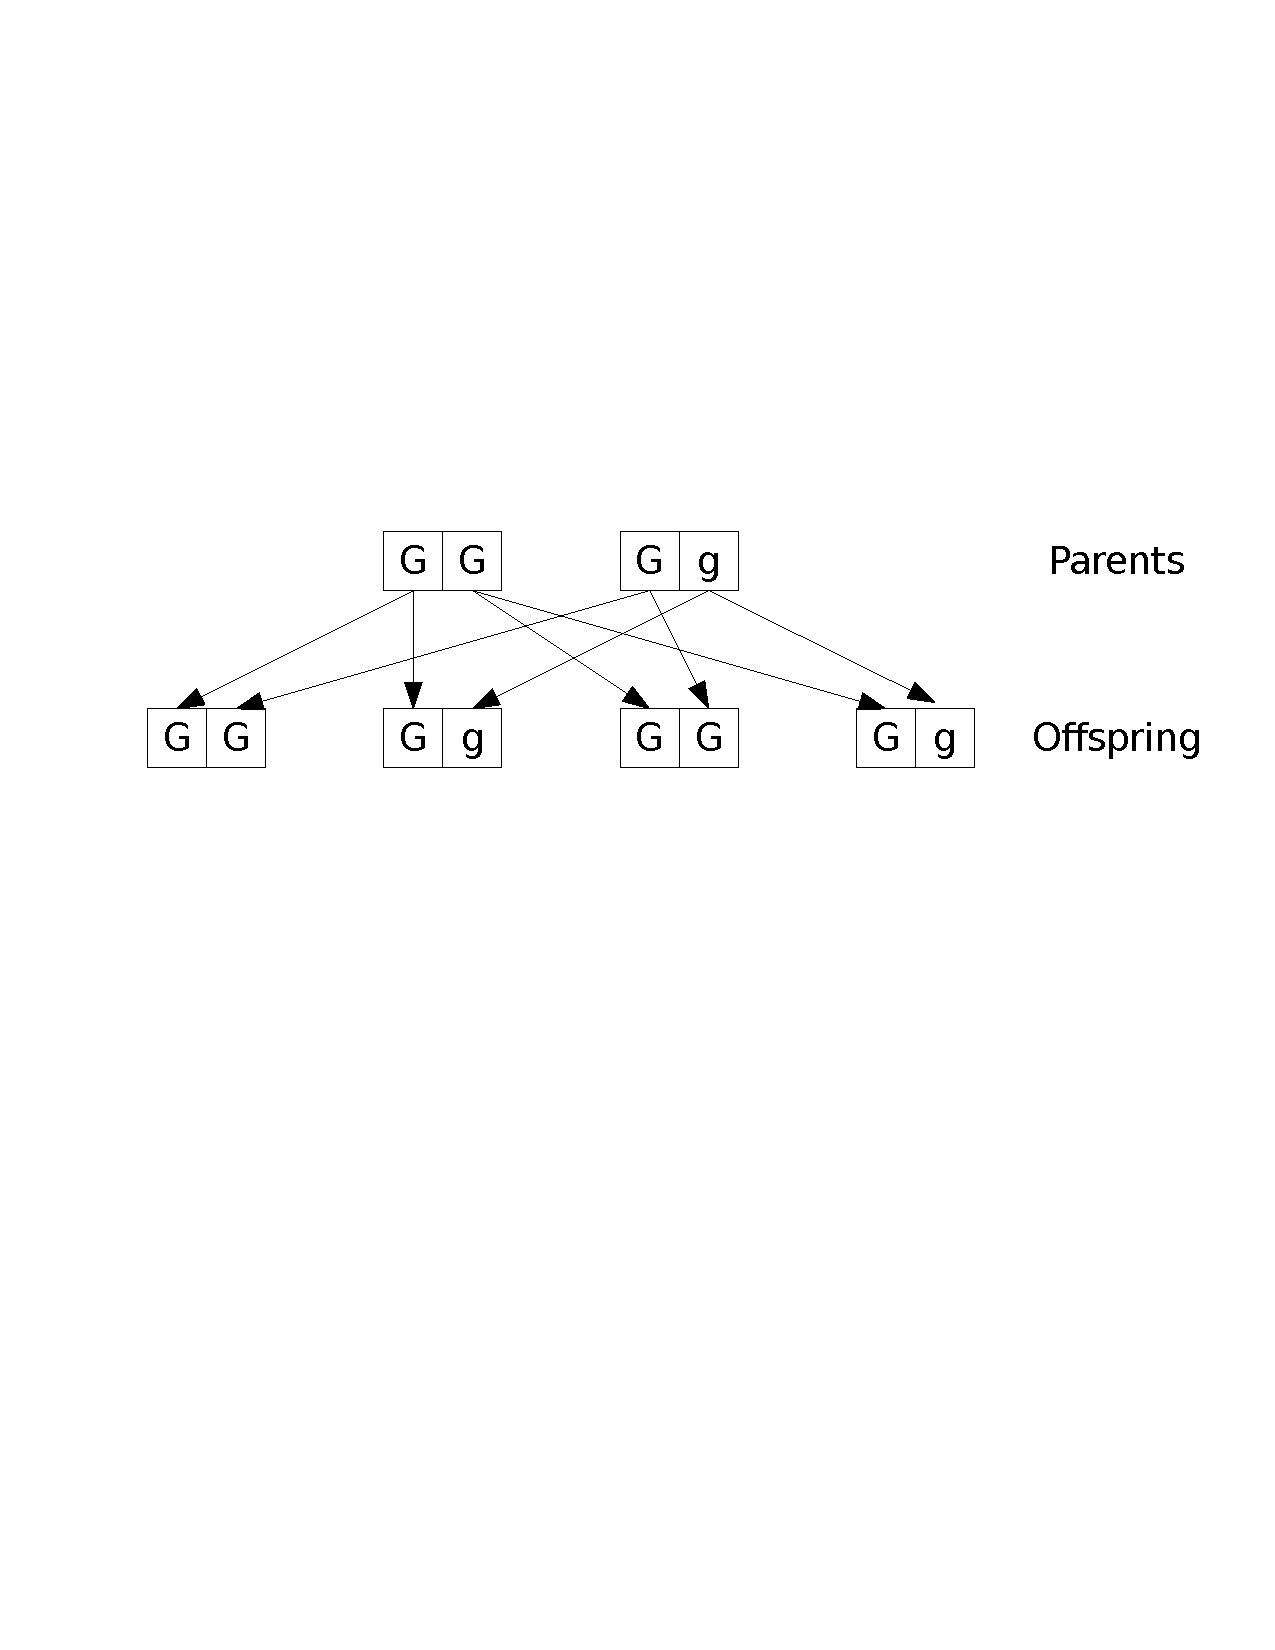
\includegraphics[width=\textwidth]{FIGS_slides/dominant_hybrid}
\end{center}
\begin{center}
\begin{tabular}{c|c}
& Parent 1 \\ 
\hline
Parent 2 &
\begin{tabular}{c|cc}
& G & G \\
\hline
G & GG & GG \\
g & Gg & Gg
\end{tabular}
\end{tabular}
\end{center}
To determine $\IP$ that offspring is of a certain type, count number of outcomes of each type (GG and Gg) and divide by 4
\vfill
$\implies$ offspring have probability
\begin{itemize}
\item $1/2$ of being GG
\item $1/2$ of being Gg
\end{itemize}
\end{frame}


\begin{frame}{Gg and Gg parents}
Both parents are hybrid
\vfill
\begin{center}
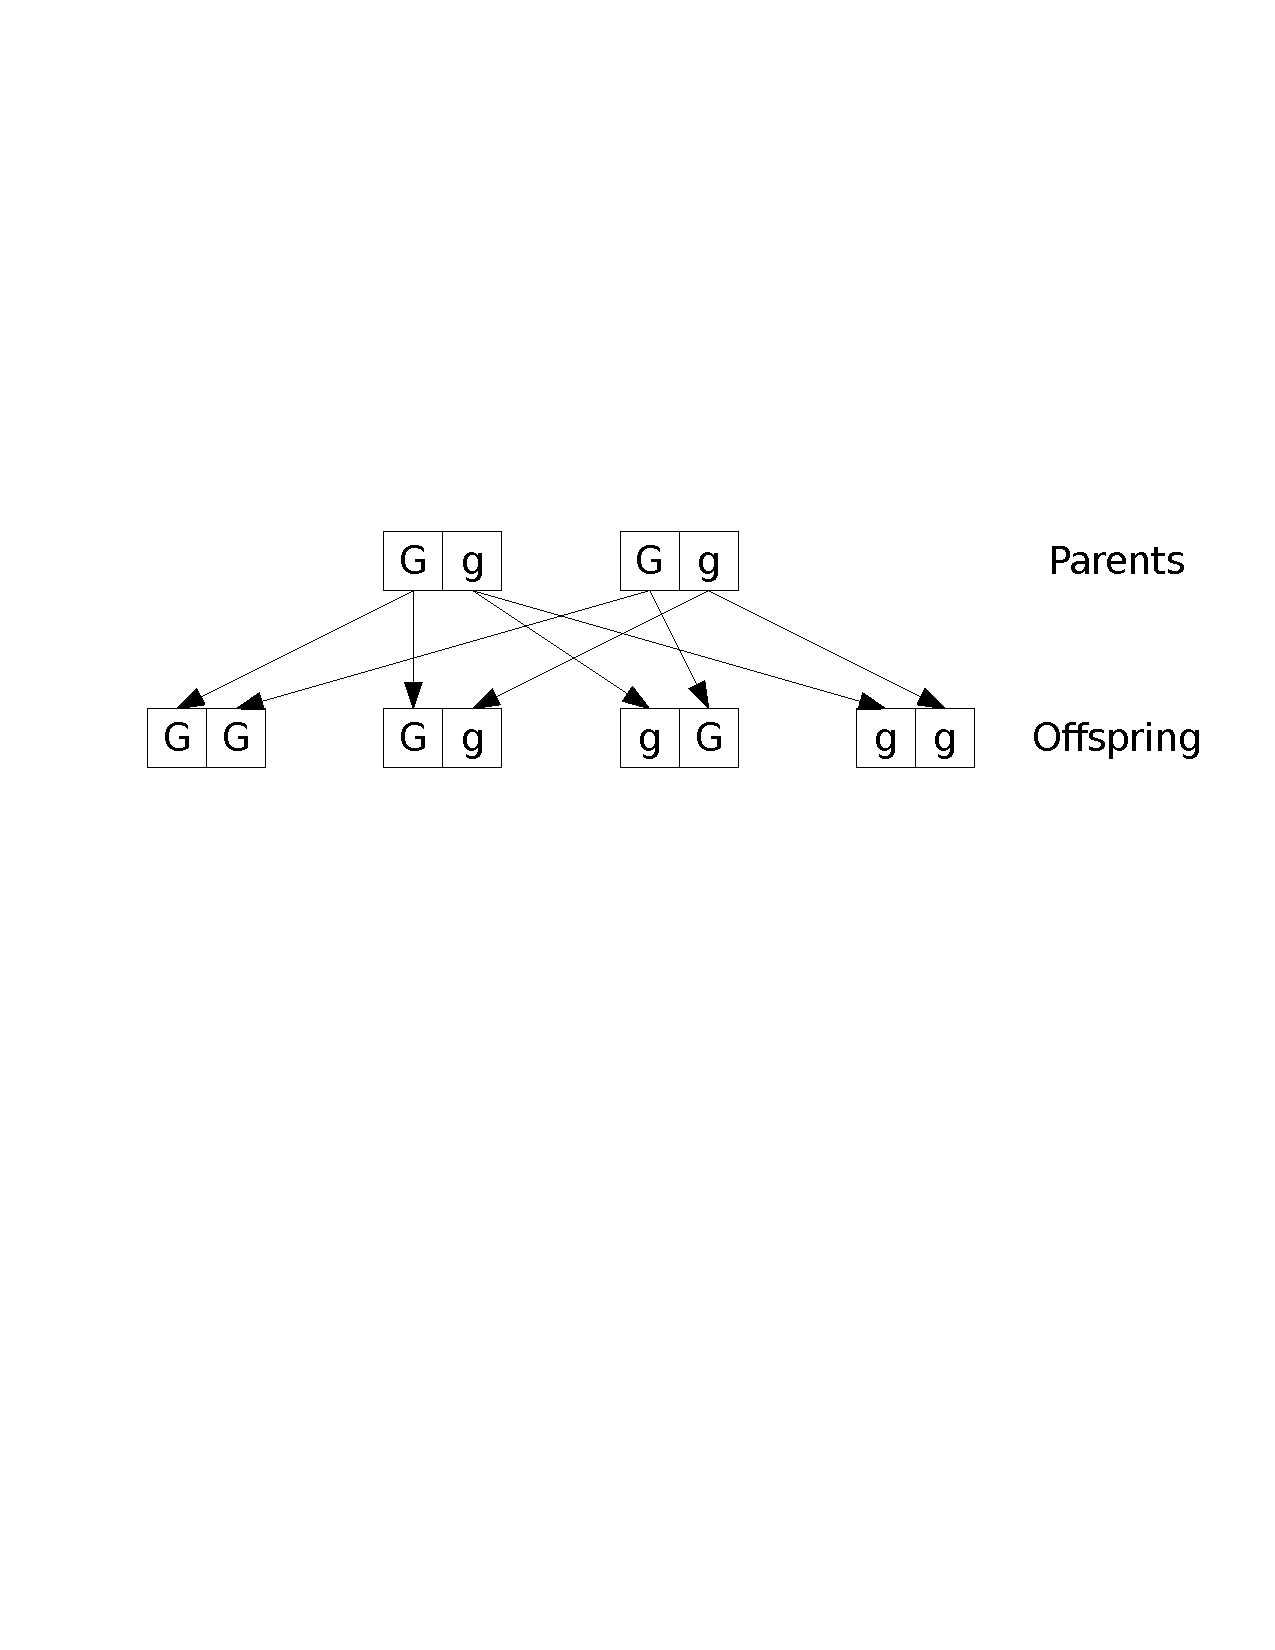
\includegraphics[width=\textwidth]{FIGS_slides/hybrid_hybrid}
\end{center}
\vfill
$\implies$ offspring have probability
\begin{itemize}
\item $1/4$ of being GG
\item $1/2$ of being Gg 
\item $1/4$ of being gg
\end{itemize}
\end{frame}


\begin{frame}{gg and Gg parents}
Recessive and hybrid parents
\vfill
\begin{center}
	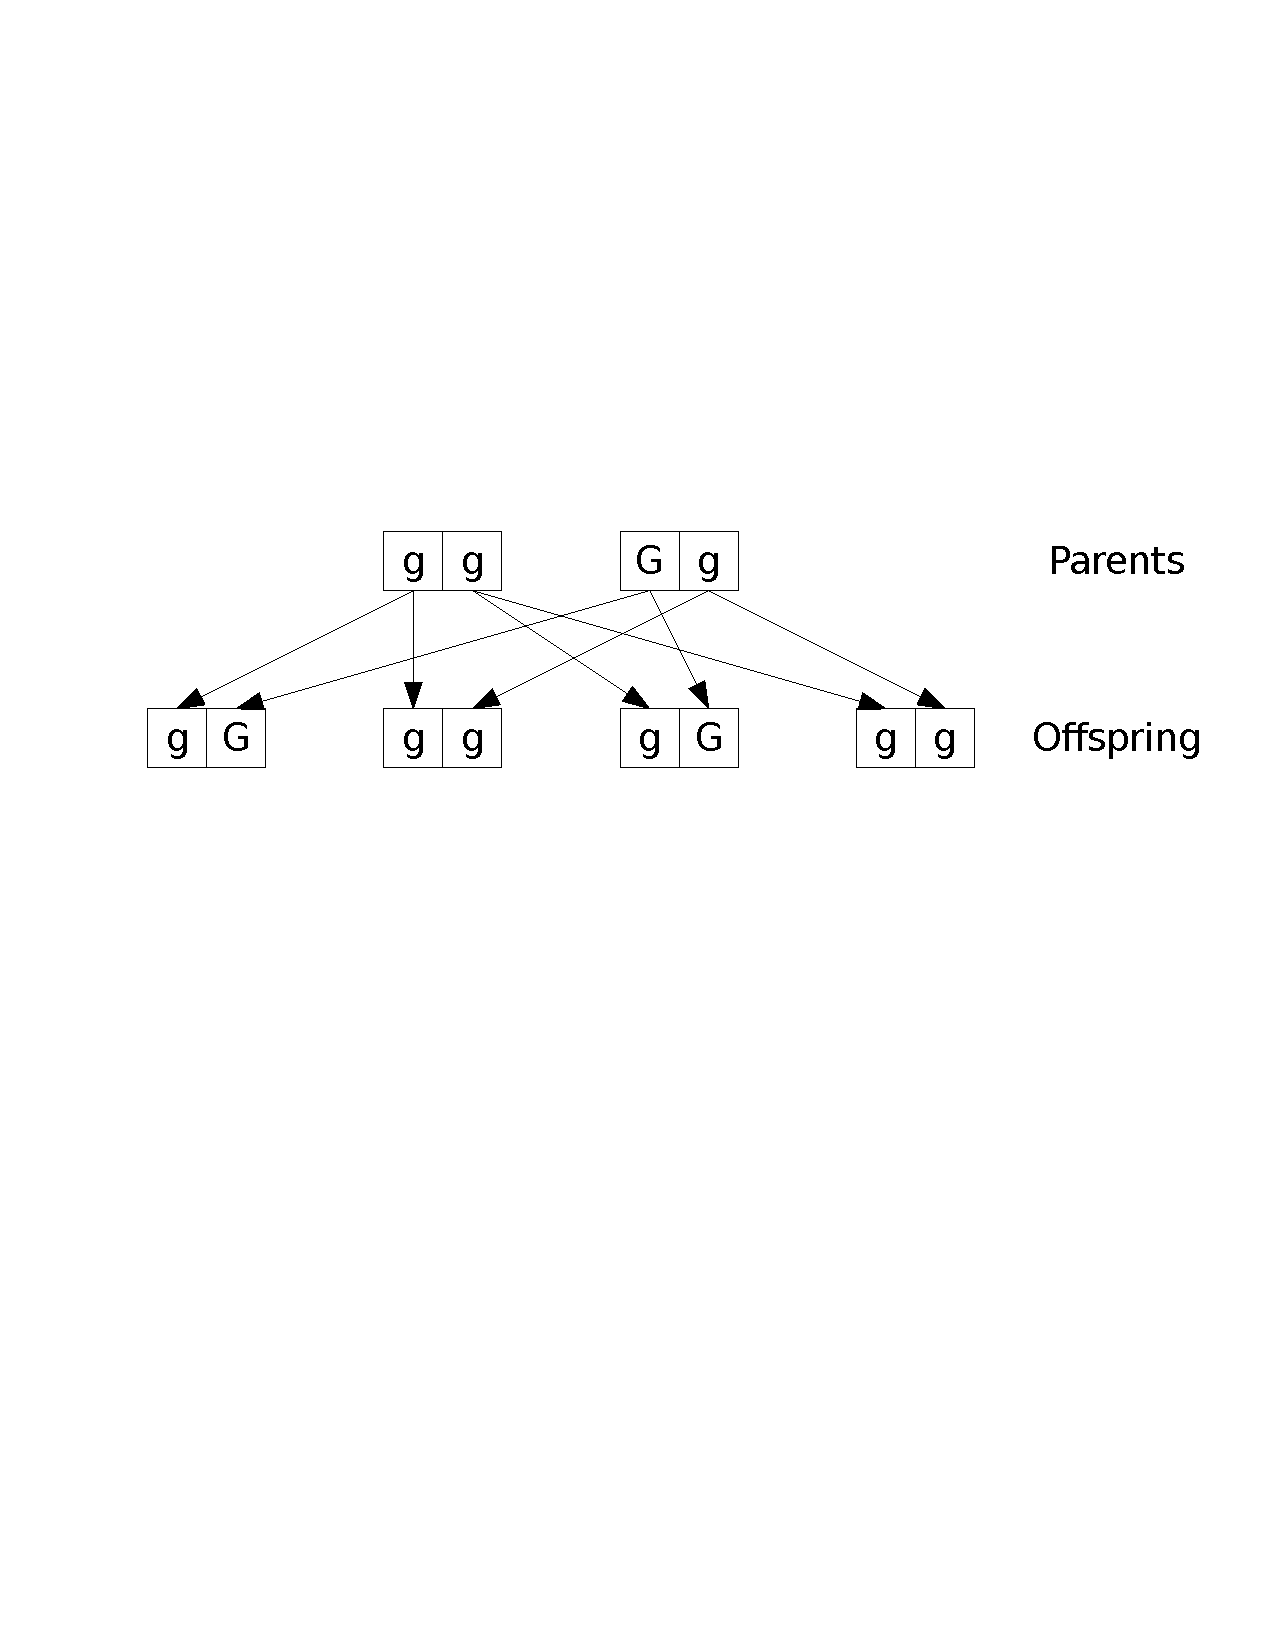
\includegraphics[width=\textwidth]{FIGS_slides/recessive_hybrid}
\end{center}
\vfill
$\implies$ offspring have probability 
\begin{itemize}
\item $1/2$ of being Gg 
\item $1/2$ of being gg
\end{itemize}
\end{frame}




%%%%%%%%%%%%%%%%%%%%
%%%%%%%%%%%%%%%%%%%%
%%%%%%%%%%%%%%%%%%%%
%%%%%%%%%%%%%%%%%%%%
\section{Repetition of the process}
\begin{frame}{General case}
$p_i(n)$: probability that state $S_i$ occurs on the $n^{th}$ repetition of the experiment, $1\leq i\leq r$
\vfill
Since one the states $S_i$ must occur on the $n^{th}$ repetition
\[
p_1(n)+p_2(n)+\cdots+p_r(n)=1
\]
$p_i(n+1)$: probability that state $S_i$, $1\leq i\leq r$, occurs on $(n+1)^{th}$ repetition of the experiment
\vfill
$r$ ways to be in state $S_i$ at step $n+1$:
\begin{enumerate}
\item Step $n$ is $S_1$. Probability of getting $S_1$ on $n^{th}$ step is $p_1(n)$, and probability of having $S_i$ after $S_1$ is $p_{1i}$. Therefore $P(S_i|S_1)=p_{1i}p_1(n)$
\item We get $S_2$ on step $n$ and $S_i$ on step $(n+1)$. Then $P(S_i|S_2)=p_{2i}p_2(n)$
\item[..]
\item[r.] Probability of occurrence of $S_i$ at step $n+1$ if $S_r$ at step $n$ is $P(S_i|S_r)=p_{ri}p_r(n)$
\end{enumerate}
\end{frame}


\begin{frame}
\begin{align*}
\implies
p_i(n+1) &= P(S_i|S_1)+\cdots+P(S_i|S_r) \\
&= p_{1i}p_1(n)+\cdots+p_{ri}p_r(n)
\end{align*}
Therefore,
\begin{align*}
p_1(n+1) &= p_{11}p_1(n)+p_{21}p_2(n)+\dots+p_{r1}p_r(n) \\
& \;\;\vdots\\
p_r(n+1) &= p_{1r}p_1(n)+p_{2r}p_2(n)+\dots+p_{rr}p_r(n)
\end{align*}
\vfill
In matrix form
\[
p(n+1)=p(n)P, \quad n=1,2,3,\dots
\]
where $p(n)=(p_1(n),p_{2}(n),\dots , p_r(n))$ is a (row) probability vector and $P=(p_{ij})$ is a $r\times r$ \emph{transition matrix},
\[
P=
\begin{pmatrix}
p_{11} & p_{12} & \cdots & p_{1r} \\
p_{21} & p_{22} & \cdots & p_{2r} \\
&&& \\
p_{r1} & p_{r2} & \cdots & p_{rr}
\end{pmatrix}
\]
\end{frame}


\begin{frame}
So
\begin{multline*}
(p_1(n+1),\ldots,p_r(n+1))  \\
=
(p_1(n),\ldots,p_r(n)) 
\begin{pmatrix}
p_{11} & p_{12} & \cdots & p_{1r} \\
p_{21} & p_{22} & \cdots & p_{2r} \\
&&& \\
p_{r1} & p_{r2} & \cdots & p_{rr}
\end{pmatrix}
\end{multline*}
\vfill
Easy to check that this gives the same expression as before
\end{frame}



\begin{frame}{Stochastic matrices}
\begin{definition}[Stochastic matrix]
The nonnegative $r\times r$ matrix $M$ is \textbf{stochastic} if $\sum_{j=1}^ra_{ij}=1$ for all $i=1,2,\dots, r$
\end{definition}
\vfill
If each row sum and each column sum equals one, the matrix is \textbf{doubly stochastic}
\vfill
\begin{theorem}\label{th:spectrum_stochastic_matrix}
Let $M$ be a stochastic matrix. Then all eigenvalues $\lambda$ of $M$ are such that $|\lambda|\leq 1$. 
Furthermore, $\lambda =1$ is an eigenvalue of $M$
\end{theorem}
\end{frame}

\begin{frame}{Long time behaviour}
Let $p(0)$ be the initial distribution (row) vector. Then
\begin{align*}
p(1) &= p(0)P \\
p(2) &= p(1)P\\
&= (p(0)P)P \\
&= p(0)P^2
\end{align*}
\vfill
Iterating, we get, for any $n$,
\[
p(n)=p(0)P^n
\]
\vfill
Therefore, 
\begin{align*}
\lim_{n\rightarrow +\infty}p(n) &=
\lim_{n\rightarrow +\infty}p(0)P^n \\
&=p(0)\lim_{n\rightarrow +\infty}P^n
\end{align*}
if this limit exists
\end{frame}


\begin{frame}
\[
\lim_{n\rightarrow +\infty}p(n) = 
p(0)\lim_{n\rightarrow +\infty}P^n
\]
Does the limit exist?
\vfill
\begin{theorem}
If $M,N$ are nonsingular stochastic matrices, then $MN$ is a stochastic matrix
\end{theorem}
\vfill
So the product of any number of stochastic matrices is also stochastic
\vfill
\begin{corollary}
If $M$ is a nonsingular stochastic matrix, then for any $k\in\IN$, $M^k$ is a stochastic matrix
\end{corollary}
\end{frame}

\section{Regular Markov chains}
\begin{frame}{Regular Markov chains}
\begin{definition}[Regular Markov chain]
A \textbf{regular} Markov chain has $P^k$ (entry-wise) positive for some integer $k>0$, i.e., $P^k$ has only positive entries
\end{definition}
\vfill
\begin{definition}[Primitive matrix]
A nonnegative matrix $M$ is \textbf{primitive} if, and only if, there is an integer $k>0$ such that $M^k$ is positive.
\end{definition}
\vfill
\begin{theorem}
Markov chain regular $\iff$ transition matrix $P$ primitive
\end{theorem}
\end{frame}

\begin{frame}{Behaviour of a regular MC}
\begin{theorem}
If $P$ is the transition matrix of a regular Markov chain, then
\begin{enumerate}
\item the powers $P^n$ approach a stochastic matrix $W$
\item each row of $W$ is the same (row) vector $w=(w_1,\ldots,w_r)$
\item the components of $w$ are positive
\end{enumerate}
\end{theorem}
\vfill
So if the Markov chain is regular
\[
\lim_{n\rightarrow +\infty}p(n)=p(0)\lim_{n\rightarrow +\infty}P^n
=p(0)W
\]
\end{frame}


\begin{frame}{Computing $W$}
If $p(n)$ converges, then $p(n+1)=p(n)P$, so $w$ is a \textbf{fixed point} of the system. Write
\[
wP=w
\]
and solve for $w$, i.e., find $w$ as left eigenvector corresponding to the eigenvalue 1
or as (right) eigenvector associated to eigenvalue 1 for the transpose of $P$
\[
P^Tw^T=w^T
\]
\vfill
$w$ might have to be normalized (you want a probability vector). Check that the norm $\|w\|$ defined by
\[
\|w\|=w_1+\cdots+w_r
\]
is equal to one. If not, use
\[
\frac{w}{\|w\|}
\]
\end{frame}

\section{Back to the genetics example}
\begin{frame}{Back to genetics}
Suppose we want to understand what it means to have hybrid individuals in the population
\vfill
Investigate this using a process of continued matings
\begin{itemize}
\item Start with an individual of known or unknown
genetic character (dominant, hybrid or recessive) and mate it with a hybrid
\item Assume that the mating results in at least one
offspring; choose one of the offspring at random and mate it with a hybrid
\item Repeat this process through a number of generations
\end{itemize}
\vfill
What can we expect in terms of the genetic composition of the population after a while? 
\vfill
$\implies$ consider MC with states GG, Gg and gg
\end{frame}


\begin{frame}
3 states: $S_1=\textrm{GG}$, $S_2=\textrm{Gg}$ and $S_3=\textrm{gg}$; we use GG, Gg and gg as well to name the states
\vfill
\begin{center}
\begin{tabular}{c|ccc}
$\nearrow$ & GG & Gg & gg \\
\hline
GG & 0.5 & 0.5 & 0 \\
Gg & 0.25 & 0.5 & 0.25 \\
gg & 0 & 0.5 & 0.5
\end{tabular}
\end{center}
\vfill
The transition probabilities are thus
\[
P=\begin{pmatrix}
\dfrac 12 & \dfrac 12 & 0 \\[10pt]
\dfrac 14 & \dfrac 12 & \dfrac 14 \\[10pt]
0 & \dfrac 12 & \dfrac 12
\end{pmatrix}
\]
\end{frame}

\begin{frame}
\[
P=\begin{pmatrix}
\dfrac 12 & \dfrac 12 & 0 \\[10pt]
\dfrac 14 & \dfrac 12 & \dfrac 14 \\[10pt]
0 & \dfrac 12 & \dfrac 12
\end{pmatrix}
\]
so
\[
P^2=\begin{pmatrix}
\dfrac 38 & \dfrac 12 & \dfrac 18 \\[10pt]
\dfrac 14 & \dfrac 12 & \dfrac 14 \\[10pt]
\dfrac 18 & \dfrac 12 & \dfrac 38
\end{pmatrix}
\]
\vfill
$\implies$ $P$ primitive $\implies$ Markov chain regular
\vfill
\begin{theorem}
$M$ primitive if the associated connection graph is strongly connected \emph{and} there is at least one positive entry on the diagonal of $M$
\end{theorem}
\end{frame}

\begin{frame}
This is checked directly on the transition graph
\vfill
\begin{center}
\begin{tikzpicture}
	[inner sep=2mm,
	place/.style={circle,draw=blue!50,fill=blue!90,thick,minimum size=1.25cm}]
	\node [place] (GG) {GG};
	\node [place] (Gg) [right=of GG] {Gg};
	\node [place] (gg) [right=of Gg]{gg};
	\draw[->] (GG) to [bend left] node [auto] {0.5} (Gg);
	\draw[->] (GG) to [loop above] node [auto] {0.5} (GG);
	\draw[->] (Gg) to [bend left] node [auto] {0.25} (GG);
	\draw[->] (Gg) to [bend left] node [auto] {0.25} (gg);
	\draw[->] (Gg) to [loop above] node [auto] {0.5} (Gg);
	\draw[->] (gg) to [bend left] node [auto] {0.5} (Gg);
	\draw[->] (gg) to [loop above] node [auto] {0.5} (gg);
\end{tikzpicture}
\end{center}
\end{frame}

\begin{frame}
Compute left eigenvector associated to 1
\[
(w_1,w_2,w_3)
\begin{pmatrix}
\frac 12 & \frac 12 & 0 \\
\frac 14 & \frac 12 & \frac 14 \\
0 & \frac 12 & \frac 12
\end{pmatrix}
=(w_1,w_2,w_3)
\]
\begin{align*}
\frac 12 w_1+\frac 14 w_2 &= w_1 \\
\frac 12 w_1+\frac 12 w_2+\frac 12 w_3 &= w_2 \\
\frac 14 w_2+\frac 12 w_3 &= w_3
\end{align*}
So $w_1=w_2/2$, $w_3=w_2/2$ and thus
\[
\frac 14 w_2+\frac 12 w_2 +\frac 14 w_2=w_2,
\]
that is, $w_2=w_2$, i.e., $w_2$ can take any value
\vfill
\[
\implies\quad w=\left(\dfrac 14,\dfrac 12,\dfrac 14\right)
\]
\end{frame}

\section{Changing the setting of the genetic experiment}
\begin{frame}
Suppose now the same type of experiment, but mate each new generation with a GG individual instead of a Gg individual
\vfill
\begin{center}
\begin{tikzpicture}
	[inner sep=2mm,
	place/.style={circle,draw=blue!50,fill=blue!90,thick,minimum size=1.25cm}]
	\node [place] (GG) {GG};
	\node [place] (Gg) [right=of GG] {Gg};
	\node [place] (gg) [right=of Gg]{gg};
	\draw[->] (GG) to [loop above] node [auto] {1} (GG);
	\draw[->] (Gg) to node [auto] {0.5} (GG);
	\draw[->] (Gg) to [loop above] node [auto] {0.5} (Gg);
	\draw[->] (gg) to node [auto] {1} (Gg);
\end{tikzpicture}
\end{center}
\vfill
\begin{minipage}{0.45\textwidth}
	\begin{center}
		\begin{tabular}{c|ccc}
		$\nearrow$ & GG & Gg & gg \\
		\hline
		GG & 1 & 0 & 0 \\
		Gg & 0.5 & 0.5 & 0 \\
		gg & 0 & 1 & 0
		\end{tabular}
	\end{center}
\end{minipage}
\begin{minipage}{0.45\textwidth}
	\[
		P=\begin{pmatrix}
		1 & 0 & 0 \\[2pt]
		\dfrac 12 & \dfrac 12 & 0 \\[7pt]
		0 & 1 & 0
		\end{pmatrix}
	\]
\end{minipage}
\begin{itemize}
\item leave gg after 1 iteration and can never return
\item when we leave Gg, we can never return
\item we can never leave GG when we get there
\end{itemize}
\end{frame}


\section{Absorbing Markov chains}
\begin{frame}{Absorbing Markov chains}
\begin{definition}[Absorbing state]
A state $S_i$ in a Markov chain is \textbf{absorbing} if whenever it occurs on the $n^{th}$ generation of the experiment, it then occurs on every subsequent step. In other words, $S_i$ is absorbing if $p_{ii}=1$ and $p_{ij}=0$ for $i\neq j$
\end{definition}
\vfill
\begin{definition}[Absorbing chain]
A Markov chain is \textbf{absorbing} if it has at least one absorbing state, and if from every state it is possible to go to an absorbing state.
In an absorbing Markov chain, a state that is not absorbing is called \textbf{transient}
\end{definition}
\end{frame}


\begin{frame}
%\begin{figure}[htbp]
%\centering
%\includegraphics[width=0.4\textwidth]{FIGS_slides/graphe_absorbant}
%\caption{Example of a graph corresponding to an absorbing Markov chain. States 1 and 4 are absorbing, states 2 and 3 are transient.}
%\label{fig:genetics_absorbing_graph}
%\end{figure}
Suppose we have a chain like the following
\begin{center}
\begin{tikzpicture}
	[inner sep=2mm,
	place/.style={circle,draw=blue!50,fill=blue!90,thick,minimum size=1cm}]
	\node [place] (1) {1};
	\node [place] (2) [right=of 1] {2};
	\node [place] (3) [right=of 2] {3};
	\node [place] (4) [right=of 3] {4};
	\draw[->] (1) to [loop above] (1);
	\draw[->] (2) to [loop above] (2);
	\draw[->] (3) to [loop above] (3);
	\draw[->] (4) to [loop above] (4);
	\draw[->] (2) to (1);
	\draw[->] (2) to [bend left] (3);
	\draw[->] (3) to [bend left] (2);
	\draw[->] (3) to (4);
\end{tikzpicture}
\end{center}
\vfill
\begin{enumerate}
\item Does the process eventually reach an absorbing state?
\item What is the average number of steps spent in a transient state, if starting in a transient state?
\item What is the average number of steps before entering an absorbing state?
\item What is the probability of being absorbed by a given absorbing state, when there are more than one, when starting in a given transient state?
\end{enumerate}
\end{frame}

\begin{frame}
The answer to the first question (``Does the process eventually reach an absorbing state?'') is given by the following result
\vfill
\begin{theorem}
In an absorbing Markov chain, the probability of reaching an absorbing state is 1
\end{theorem}
\end{frame}

\begin{frame}
To answer the other questions, write the transition matrix in \textbf{standard} form
\vfill
For an absorbing chain with $k$ absorbing states and $r-k$ transient states, write transition matrix as
\[
P=\begin{pmatrix}
\mathbb{I}_k & \mathbf{0} \\
R & Q
\end{pmatrix}
\]
with following meaning
\begin{center}\footnotesize
\begin{tabular}{ccc}
& Absorbing states & Transient states \\
Absorbing states & $\mathbb{I}_k$ & $\mathbf{0}$ \\
Transient states & $R$ & $Q$
\end{tabular}
\end{center}
with $\mathbb{I}_k$ the $k\times k$ identity matrix, $\mathbf{0}$ an $k\times(r-k)$ matrix of zeros, $R$ an $(r-k)\times k$ matrix and $Q$ an $(r-k)\times(r-k)$ matrix.
The matrix $\mathbb{I}_{r-k}-Q$ is invertible. Let
\begin{itemize}
\item $N=(\mathbb{I}_{r-k}-Q)^{-1}$ the \textbf{fundamental matrix} of the MC
\item $T_i$ sum of the entries on row $i$ of $N$
\item $B=NR$
\end{itemize}
\end{frame}

\begin{frame}
Answers to our remaining questions:
\vfill
\begin{enumerate}
\setcounter{enumi}{1}
\item $N_{ij}$ average number of times the process is in the $j$th transient state if it starts in the $i$th transient state
\vfill
\item $T_i$ average number of steps before the process enters an absorbing state if it starts in the $i$th transient state
\vfill
\item $B_{ij}$ probability of eventually entering the $j$th absorbing state if the process starts in the $i$th transient state
\end{enumerate}
\vfill
\end{frame}

\begin{frame}{Back to the genetic example}
The matrix is already in standard form
\[
P=\left (
\begin{array}{ccc}
1 & 0 & 0 \\
\frac 12 & \frac 12 & 0 \\
0 & 1 & 0
\end{array}\right)
=\begin{pmatrix}
\mathbb{I}_1 & \mathbf{0} \\
R & Q
\end{pmatrix}
\]
with $\mathbb{I}_1=1$, $\mathbf{0}=(0\;\; 0)$ and
\[
R=\begin{pmatrix}
\frac 12\\ 0
\end{pmatrix}
\qquad
Q=\begin{pmatrix}
\frac 12 & 0\\
1 & 0
\end{pmatrix}
\]
We have
\[
\mathbb{I}_2-Q=\begin{pmatrix}
1 & 0 \\
0 & 1
\end{pmatrix}
-\begin{pmatrix}
\frac 12 & 0\\
1 & 0
\end{pmatrix}
=\begin{pmatrix}
\frac 12 & 0\\
-1 & 1
\end{pmatrix}
\]
so
\[
N=(\mathbb{I}_2-Q)^{-1}=
2\begin{pmatrix}
1 & 0 \\
1 & \frac 12
\end{pmatrix}=
\begin{pmatrix}
2 & 0 \\
2 & 1
\end{pmatrix}
\]
Then
\[
T=N\nbOne=\begin{pmatrix}
2\\
3
\end{pmatrix}
\]
and
\[
B=NR=
\begin{pmatrix}
2 & 0 \\
2 & 1
\end{pmatrix}
\begin{pmatrix}
\frac 12\\ 0
\end{pmatrix}
=
\begin{pmatrix}
1\\ 1
\end{pmatrix}
\]
\end{frame}


\begin{frame}
\begin{enumerate}
\setcounter{enumi}{1}
\item $N_{ij}$ average number of times the process is in the $j$th transient state if it starts in the $i$th transient state
\[
N=
\begin{pmatrix}
2 & 0 \\
2 & 1
\end{pmatrix}
\]
\vfill
\item $T_i$ average number of steps before the process enters an absorbing state if it starts in the $i$th transient state
\[
T=\begin{pmatrix}
2\\
3
\end{pmatrix}
\]
\vfill
\item $B_{ij}$ probability of eventually entering the $j$th absorbing state if the process starts in the $i$th transient state
\[
B
\begin{pmatrix}
1\\ 1
\end{pmatrix}
\]
\end{enumerate}
\vfill
\end{frame}



\end{document}
